We showed how the proposed MoC could be modelled in AGREE annex explicitly. However, this could be done behind the scene by the translator.
We propose a new AGREE usage flow, where a user has to choose the desired MoC (synchronous or scheduled AGREE) under which the contracts are to be verified. The choice of MoC is inspired by the concept of \emph{director} adopted in the Ptolemy project \cite{Ptolemy}. If the scheduled AGREE MoC is chosen, the user also needs to specify a schedule. Then, the AGREE translator will generate the corresponding Lustre model reflecting the desired semantics. AGREE uses a variant of Lustre \cite{GAO2008111} language. It introduced an expression called \emph{condact} to clock nodes, i.e. \emph{Condact (clock, node\_name(), initial\_output)}. It is essential to our backend modelling. A clocked node updates the local and output signals when the clock is true, otherwise it keeps the previous value of the local and output signals. We are aware that more recent Lustre developement introduced similar temporal operators like \emph{when} and \emph{current}. We use \emph{condact} simply because it is supported by the underlying SMT solver.

In AGREE backend, each AADL thread is translated to a Lustre node, as shown in Figure \ref{WPMlustre}. Note that the translation uses a \emph{constraint} style, where thread outputs are mapped to the node inputs. This means that the \emph{condact} expression does not directly clock the thread outputs. We add a Lustre assertion for each thread output to enforce the clock semantics. Figure \ref{lustreAsync} shows an example of the usage of \emph{condact} with assertions. Note that we use the \emph{complete} event to clock the node.  

\begin{figure}[ht!]
\centering
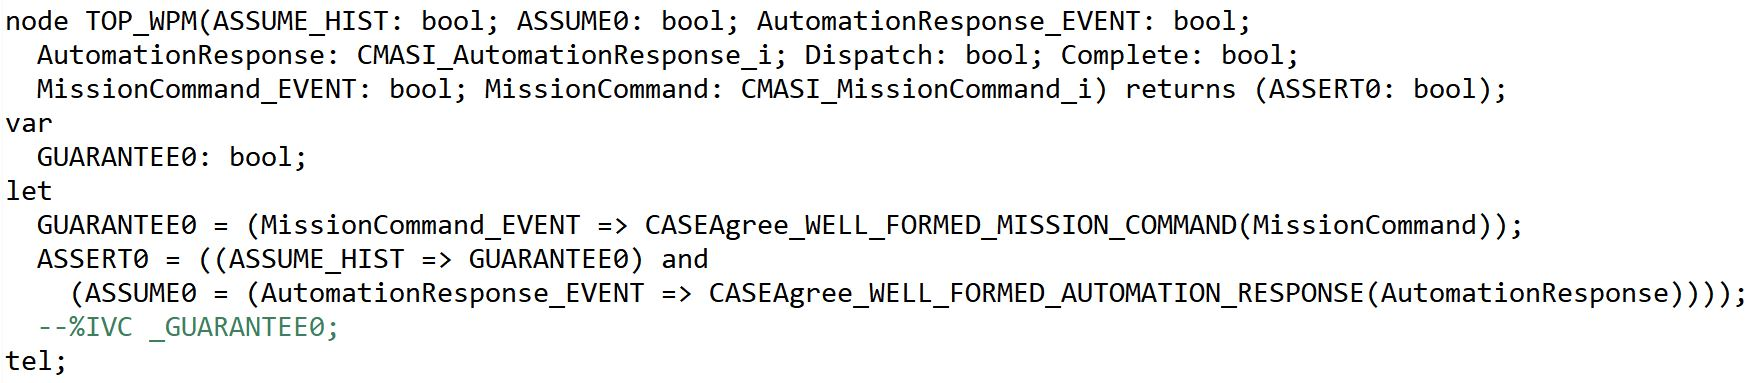
\includegraphics[width=120mm]{wpmLustre2.jpg}
\caption{A Lustre Model of AADL Thread \label{WPMlustre}}
\end{figure}

\begin{figure}[ht!]
\centering
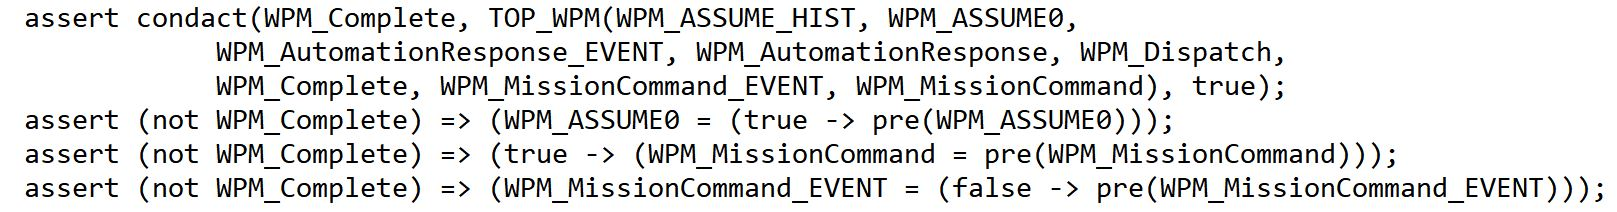
\includegraphics[width=120mm]{lustreAsync4.jpg}
\caption{A Lustre expression \emph{condact} Usage Example\label{lustreAsync}}
\end{figure}

During the translation, operator \emph{pre} needs to be handled carefully. It is interpreted as previous \emph{tick} in synchronous AGREE MoC. However, in the scheduled AGREE MoC, we interpret it as the previous \emph{activation}. If the operator is applied to a thread output or local variable, its semantics is enforced by the assertion on the output or the \emph{condact} expression, respectively. If the operator is applied to a thread input, we introduce a local variable, assigned to the input value. Due to the \emph{condact} semantics, the local variable represents the clocked input. And it is used to replace the input in a \emph{pre} expression.

%\begin{figure}[ht!]
%\centering
%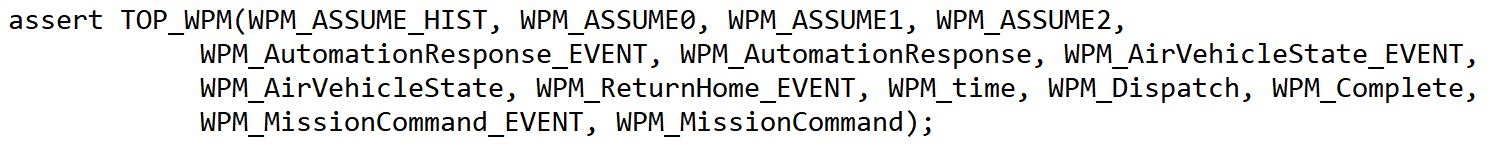
\includegraphics[width=120mm]{lustreSync2.jpg}
%\caption{An AADL Model Illustrating Motivation\label{lustreSync}}
%\end{figure}

%\begin{lstlisting}[language=c,frame=single,caption=An AGREE model of a schedule,label=schedule_model]
%  assert condact(WPM__Complete, _TOP__WPM(WPM____ASSUME__HIST, WPM____ASSUME0, WPM____ASSUME1, WPM____ASSUME2, 
%				WPM__AutomationResponse___EVENT_, WPM__AutomationResponse, WPM__AirVehicleState___EVENT_, WPM__AirVehicleState, 
%                WPM__ReturnHome___EVENT_, WPM__time, WPM__Dispatch, WPM__Complete, WPM__MissionCommand___EVENT_, WPM__MissionCommand), true);
%  assert (not WPM__Complete) => (WPM____ASSUME0 = (true -> pre(WPM____ASSUME0)));
%  assert (not WPM__Complete) => (WPM____ASSUME1 = (true -> pre(WPM____ASSUME1)));
%  assert (not WPM__Complete) => (WPM____ASSUME2 = (true -> pre(WPM____ASSUME2)));
%  assert (not WPM__Complete) => (true -> (WPM__MissionCommand = pre(WPM__MissionCommand)));
%  assert (not WPM__Complete) => (WPM__MissionCommand___EVENT_ = (false -> pre(WPM__MissionCommand___EVENT_)));
%\end{lstlisting}  
  
%In AGREE backend translation, a thread is translated as a node with constraints on thread input and output values. All thread inputs and outputs are mapped to the inputs of a node. The \emph{condact} expression does not constrain the values of the inputs of the corresponding node. Thus, we need to use additional assertions to ensure that the output of a thread updates value only when \emph{Complete} is true, otherwise keeps its previous value. That is, \emph{assert (not complete) => (Output = (0 -> pre(Output)));}

%Condact (clock, node_name(), initial_output)
%It computes node local variables and outputs when the clock is true, and holds the previous values when false.
%Propose: use condact to model AADL threads
%Lustre code: assert(condact(Complete, Thread_node(in, out,…), true));
%It matches AGREE semantics
%Contracts only hold @Complete
%Local variables are updated only once per cycle (@Complete)
